\documentclass[a4paper,11pt]{article}
\usepackage[utf8]{inputenc}
\usepackage[T1]{fontenc}
\title{Universidade Federal do Rio Grande do Norte\\Métodos Computacionais em Engenharia - T01\linebreak\linebreak\linebreak\linebreak  Aplicação dos métodos de Runge-Kutta de 4ª e 6ª ordem para a resolução de Equações  Diferenciais Ordinárias de 2ª ordem}
\author{}
\date{}
\usepackage{amsmath}
\usepackage{float}
\usepackage{ae}
\usepackage[brazil]{babel}
\usepackage{indentfirst}
\usepackage{url}
\usepackage{graphicx}
\usepackage[autostyle]{csquotes}
\graphicspath{ {./images/} }
\usepackage{hyperref}
\usepackage{verbatim}
\usepackage{minted}
\usepackage[
    style=numeric,
    sorting=none,
    maxbibnames=10]{biblatex}
\addbibresource{referencia.bib}
\makeindex
%%%
%%%
\begin{document}
\maketitle
\thispagestyle{empty}
\vspace{2cm}
\begin{minipage}{\textwidth}
\flushright
{\large
Grupo 4:\\
Alan Lima de Medeiros\\
Clayton Rylmer Paiva Maia de Almeida\\
Enzo Hêndrio Gomes Araújo\\
João Lucas Freitas Dantas Borges\\

\vspace{0.5cm}
\vspace{0.5cm}

Docente:\\
Paulo Sérgio da Motta Pires\\}
\vspace{3.5cm}
\center
{\large
Natal-RN\\06/2022}
\end{minipage} 
\pagebreak

\tableofcontents

\pagebreak

\section{Introdução}
    O presente trabalho tem como objetivo aplicar os métodos de Runge-Kutta de 4ª (RK4) e 6ª (RK6) ordem para se resolver uma Equação Diferencial Ordinária de 2ª Ordem (EDO2). Em síntese, os métodos citados compreendem parte de um grupo de técnicas iterativas para a resolução numérica de Equações Diferenciais Ordinárias (EDO).  
    
    Sob essa perspectiva, esses métodos utilizam equações bem estabelecidas para se tentar encontrar uma solução aproximada da EDO em questão. Desse modo, para o RK4, os elementos do conjunto solução são encontrados pela equação abaixo.
    
    \begin{equation}
        \label{RK4}
        y_{n+1} = y_n + \frac{1}{6}(k_1+2k_2+2k_3+k_4)
    \end{equation}
    
    Onde os termos $k_1$, $k_2$, $k_3$ e $k_4$ são encontrados pelas equações:
    
    \begin{equation}
        \label{K1}
        k_1=hz_n
    \end{equation}
    \begin{equation}
        \label{K2}
        k_2=h\left(z_n+\frac{l_1}{2}\right)
    \end{equation}
    \begin{equation}
        \label{K3}
        k_3=h\left(z_n+\frac{l_2}{2}\right)
    \end{equation}
    \begin{equation}
        \label{K4}
        k_4=h(z_n+l_3)
    \end{equation}
    
    Pelas equações de 2 a 5, observa-se que aparecem os termos $z_n$, $l_1$, $l_2$ e $l_3$. Isso se dá, pois ao se trabalhar com uma EDO2, faz-se necessário separar a equação de segunda ordem em duas de primeira ordem. Sendo assim, essas componentes representam uma dessas equações e seus valores podem ser encontrados pelas equações:
    \begin{equation}
        \label{zn}
        z_{n+1} = z_n + \frac{1}{6}(l_1+2l_2+2l_3+l_4)
    \end{equation}
        \begin{equation}
        \label{l1}
        l_1=hf(x_n,y_n)
    \end{equation}
    \begin{equation}
        \label{l2}
        l_2=hf\left(x_n+\frac{h}{2},y_n+\frac{k_1}{2}\right)
    \end{equation}
    \begin{equation}
        \label{l3}
        l_3=hf\left(x_n+\frac{h}{2},y_n+\frac{k_2}{2}\right)
    \end{equation}
    \begin{equation}
        \label{l4}
        l_4=hf(x_n+h,y_n+k_3)
    \end{equation}
    
    O termo h que aparece em praticamente todas as equações representa a distância entre os valores do eixo das abscissas e a função $f(x,y)$ é a função em análise.
    
    
    Analogamente, o RK6 utiliza equações similares, como se pode observar pelas equações abaixo:
    
    \begin{equation}
        \label{RK6}
        y_{n+1} = y_n + hz_n \frac{1}{90}(7k_0+24k_1+6k_2+8k_3)
    \end{equation}
    \begin{equation}
        \label{zn6}
        z_{n+1} = z_n + \frac{1}{90h}(7k_0+32k_1+12k_2+32k_3+7k_4)
    \end{equation}
    
    Onde os coeficientes $k_0$, $k_1$, $k_2$, $k_3$ e $k_4$ são quantificados por:
    
    \begin{equation}
        \label{k_0}
        k_0=h^2f(x_n,y_n)
    \end{equation}
    \begin{equation}
        \label{k_1}
        k_1=h^2f\left(x_n+\frac{1}{4}h,y_n+\frac{1}{4}hz_n+\frac{1}{32}k_0\right)
    \end{equation}
    \begin{equation}
        \label{k_2}
        k_2=h^2f\left(x_n+\frac{1}{2}h,y_n+\frac{1}{2}hz_n-\frac{1}{24}k_0+\frac{1}{6}k_1\right)
    \end{equation}
    \begin{equation}
        \label{k_3}
        k_3=h^2f\left(x_n+\frac{3}{4}h,y_n+\frac{3}{4}hz_n+\frac{3}{32}k_0+\frac{1}{8}k_1+\frac{1}{16}k_2\right)
    \end{equation}
    \begin{equation}
        \label{k_4}
        k_4=h^2f\left(x_n+h,y_n+hz_n+\frac{3}{7}k_1-\frac{1}{14}k_2+\frac{1}{7}k_3\right)
    \end{equation}
    
    Cabe ressaltar que ambos os métodos necessitam de condições iniciais, sendo elas para uma EDO2 um valor inicial para a função e outro para a sua derivada primeira. Além disso, o que diferencia um método do outro é o grau de precisão. Essa diferença se acentua a medida que o $h$ aumenta, de forma que, para $h$ muito pequeno, os dois métodos basicamente são equivalentes em termos de resultados. 
    
    
    Para além disso, os resultados podem divergir ainda mais, computacionalmente, a depender do tipo de precisão utilizada para os cálculos. A precisão simples faz uso de 32 bits para representar um número em ponto flutuante, enquanto a precisão dupla utiliza 64 bits. Nesse sentido, quanto maior a precisão, maior será o grau de certeza da representação de um número. Para o escopo deste projeto, apenas a precisão dupla (64 bits) será trabalhada.
\pagebreak

\section{Metodologia}

    O desenvolvimento deste projeto se deu em meio a aplicação da metodologia ágil Scrum. Dessa forma, o grupo de desenvolvedores se reuniu visando planejar as atividades que seriam realizadas para se atingir o resultado final dentro do prazo estabelecido. Após o refinamento do backlog, estipulou-se que o Menor Produto Viável (MVP) deveria ser construído em duas sprints de uma semana cada. O cronograma do projeto pode ser visualizado na figura \ref{cronograma}.
    
    \begin{figure}[H]
        \centering
        \makebox[\textwidth]{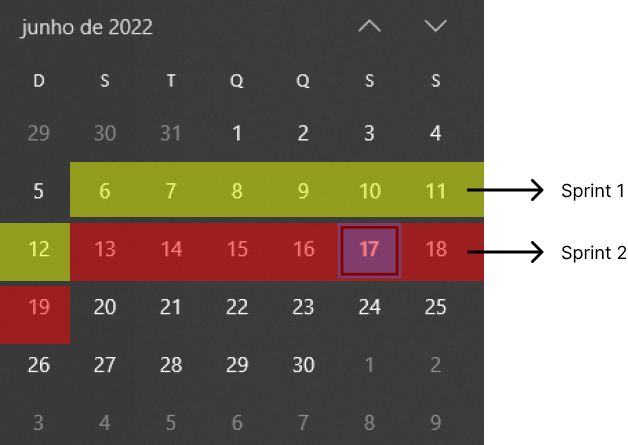
\includegraphics[scale=0.35]{images/Group 1.png}}
        \caption[width=\columnwidth]{Cronograma.}
        \label{cronograma}
    \end{figure}
    
    A organização dessas sprints foi feita com o aplicativo de gerenciamento de projetos Trello, figura \ref{Trello}. Nesse software, as atividades para cada sprint foram criadas e, dessa maneira, confirmou-se que para a primeira sprint ficariam as atividades de separação das equações diferenciais, a resolução utilizando o software de planilhas Excel e a linguagem de programação Python, bem como seriam feitos os gráficos e análises das soluções encontradas.
    
    \begin{figure}[H]
        \centering
        \makebox[\textwidth]{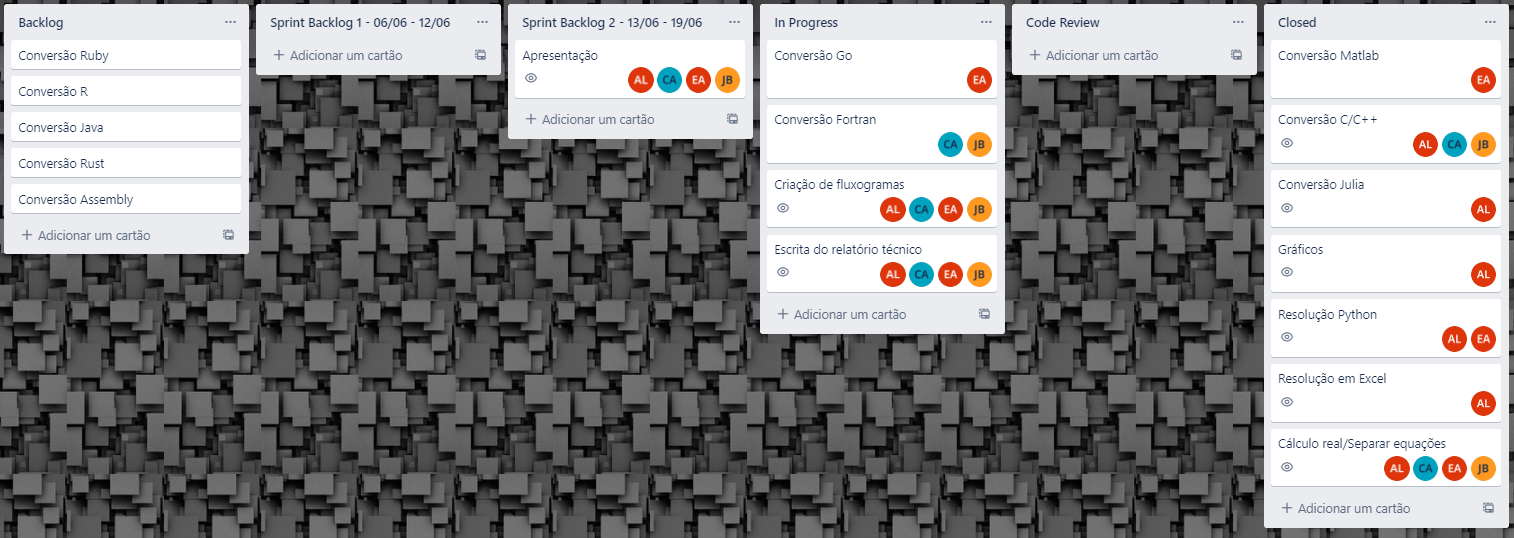
\includegraphics[scale=0.36]{images/shot_220617_224554.png}}
        \caption[width=\columnwidth]{Gerenciador de projetos.}
        \label{Trello}
    \end{figure}
    
    Complementarmente, a segunda sprint seria reservada para se converter o código feito em Python para outras linguagens de programação como C++, Julia e Matlab, utilizando a IDE Visual Studio Code (VSCode) e/ou repl.it. Ademais, nessa etapa o relatório técnico e a apresentação também seriam feitos. 
    
    
    Diante disso, separou-se primeiramente a equação diferencial de 2ª ordem em duas equações de 1ª ordem. Em seguida, a solução foi encontrada utilizando o Excel, visando facilitar a visualização dos cálculos e garantir, graficamente, os resultados obtidos em um primeiro momento. Após isso, o ambiente Colab foi utilizado para se desenvolver a solução em Python, na versão 3.7.13 e com precisão dupla. Como resultado, obteve-se um notebook Python contendo as soluções do RK4 e RK6, bem como as análises gráficas.
    
    
    Aproveitando-se desse código, construiu-se uma aplicação Python e se colocou esse aplicativo em um servidor WEB, chamado Streamlit, para que se tivesse uma resolução mais interativa.
    
    
    Por fim, o relatório foi escrito em LaTeX no editor de texto Overleaf, objetivando manter o padrão de desenvolvimento em nuvem, garantindo maior segurança no armazenamento do trabalho e integração da equipe no processo. O fluxo completo pode ser visto na figura \ref{fluxo}.
    
    \begin{figure}[H]
        \centering
        \makebox[\textwidth]{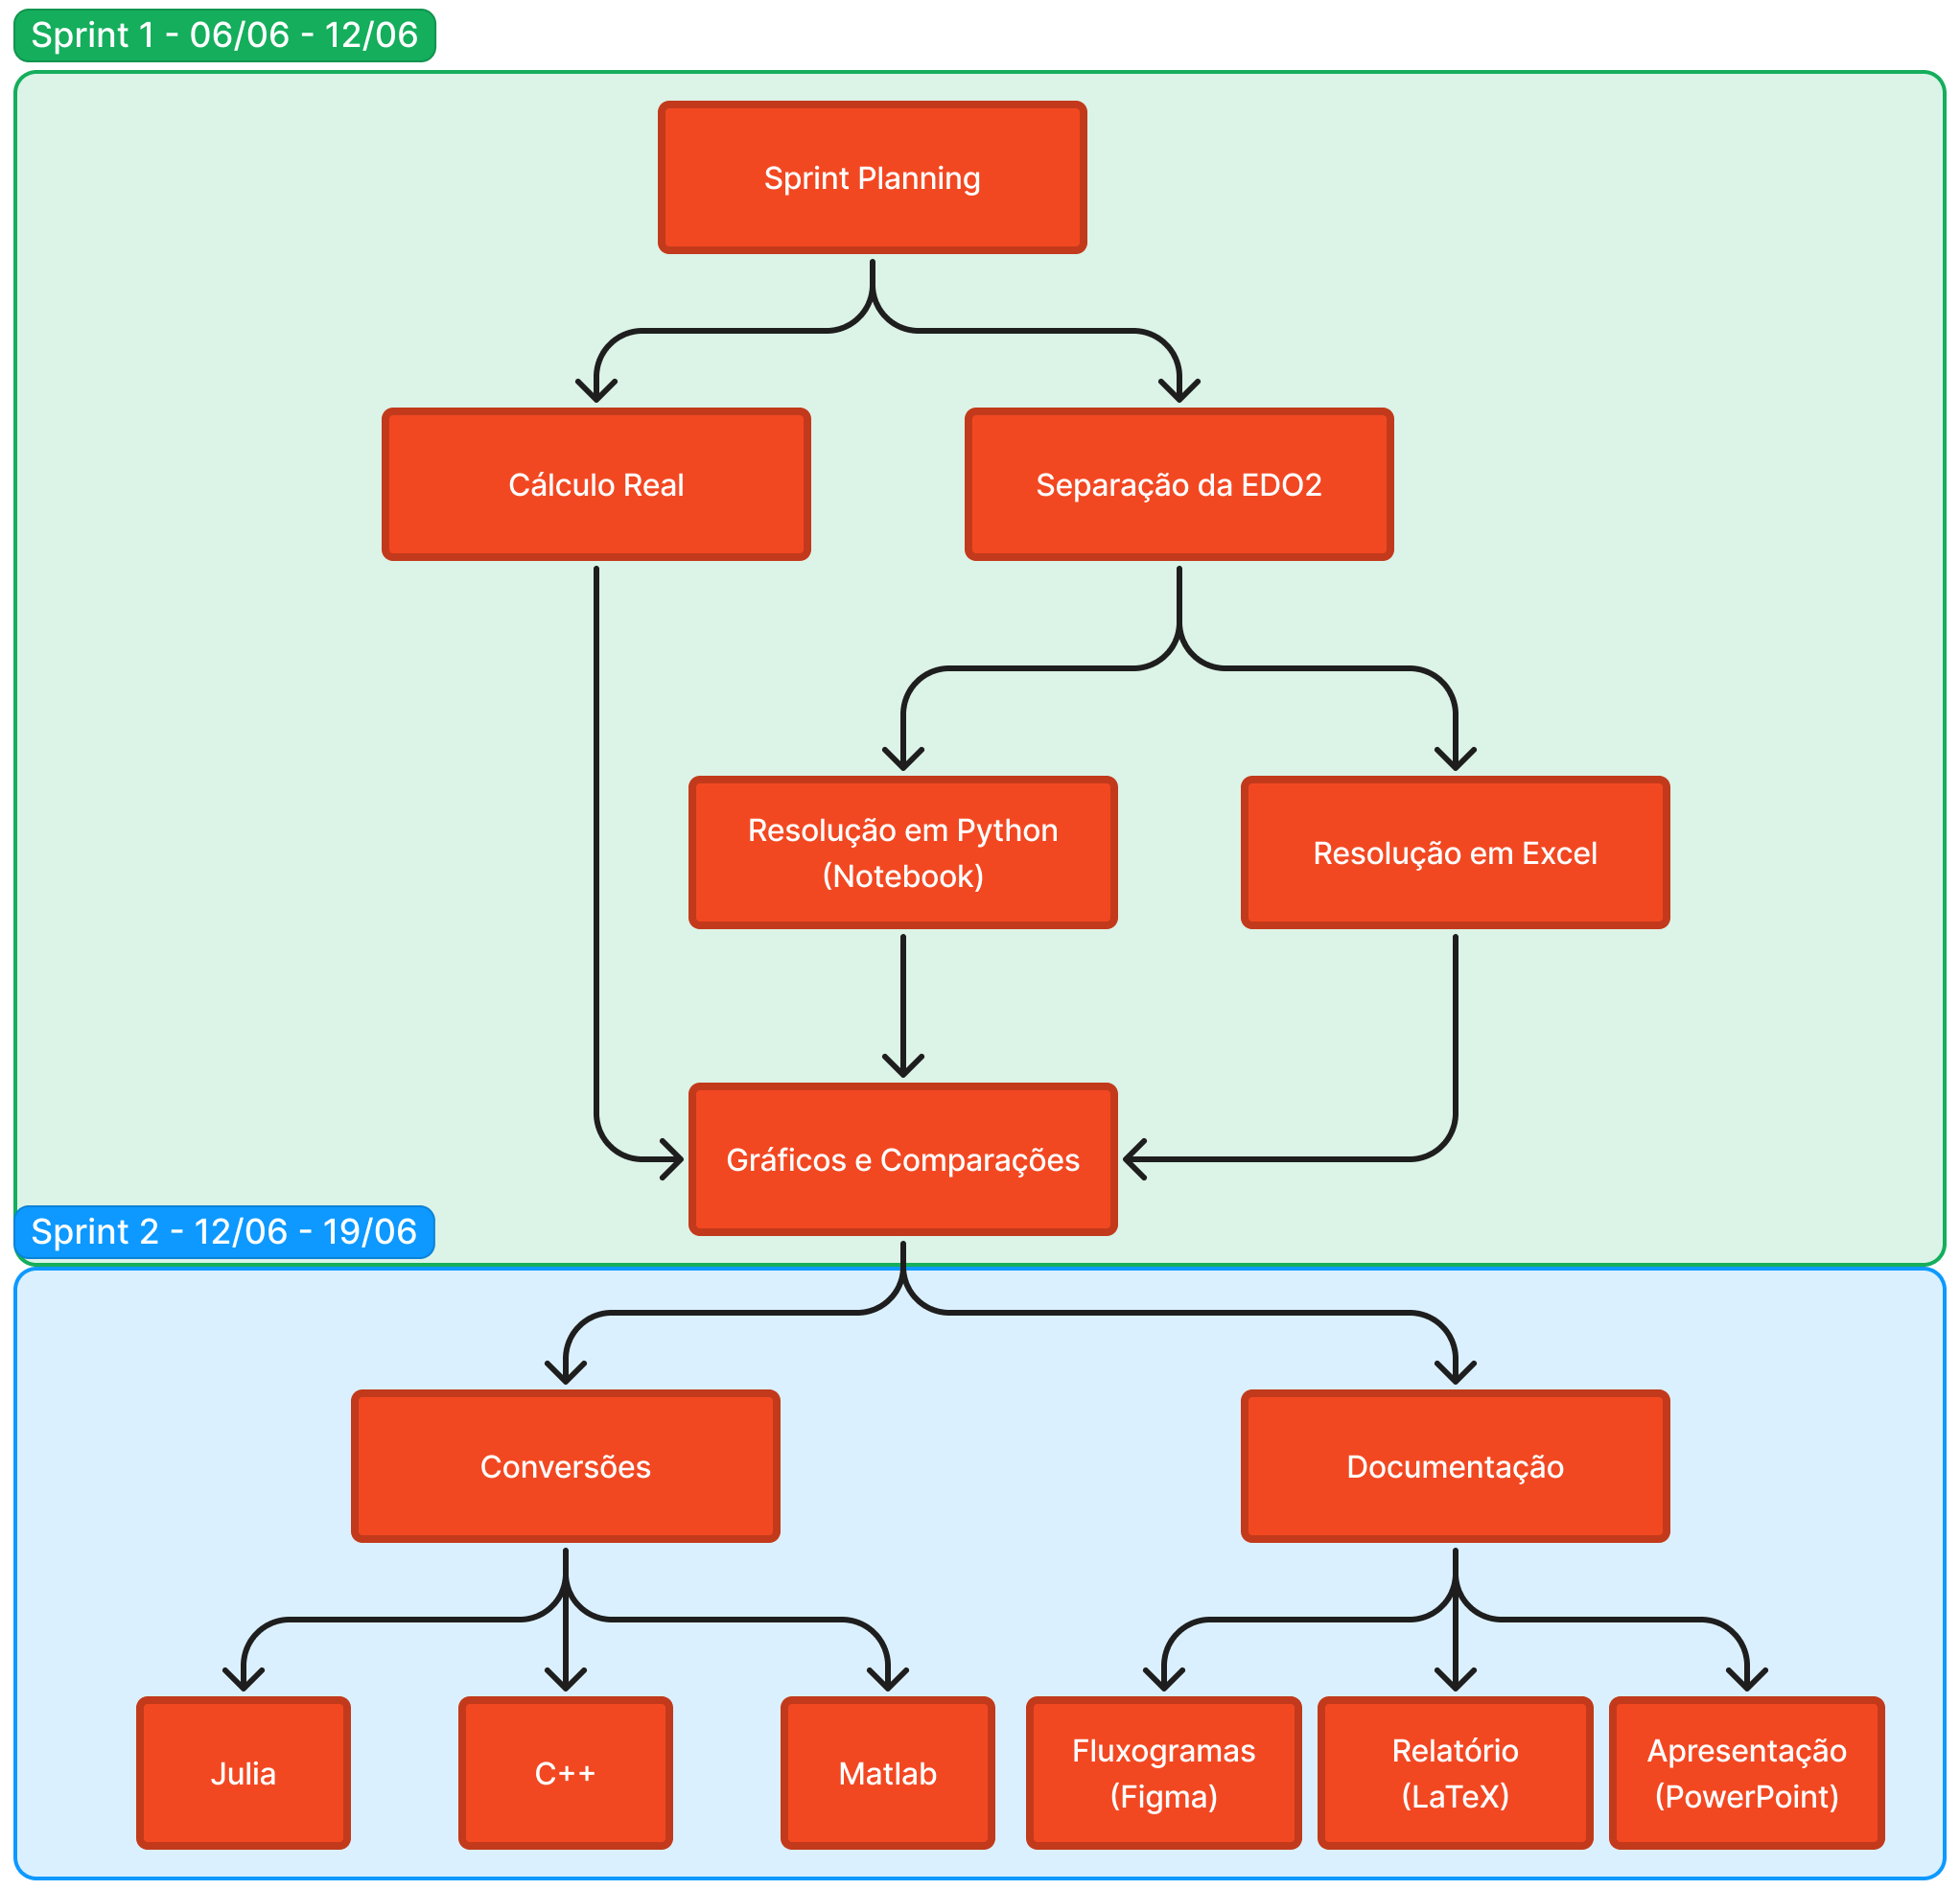
\includegraphics[scale=0.3]{images/Untitled.png}}
        \caption[width=\columnwidth]{Fluxo do projeto.}
        \label{fluxo}
    \end{figure}
    
\pagebreak

\section{Problema}

    O problema em questão fornecia uma EDO2, equação \ref{EDO2}, e solicitava que soluções fossem encontradas pelos métodos de RK4 e RK6 para cada $h$ pedido. O h poderia assumir os valores de 0.025, 0.25 e 0.5.
    
    \begin{equation}
        \label{EDO2}
        \frac{d^2y(x)}{dx^2}=-\left(100+\frac{1}{x^2}\right)y(x)=f(x,y)
    \end{equation}
    
    Além disso, as condições iniciais, $y(1)=-0.24593576$ e $y'(1)=-0.55769344$, e o intervalo, de 1 a 10$\pi$, foram fornecidos. Diante disso, a equação \ref{EDO2} foi manipulada da seguinte forma:
    
    \begin{equation}
        \label{z}
        z=y' \rightarrow z(1)=y'(1)=-0.55769344
    \end{equation}
    \begin{equation}
        \label{y}
        z'=y''=-\left(100+\frac{1}{x^2}\right)y(x)
    \end{equation}
    
\subsection{Resolução: Excel}

    Em excel, foram-se criadas 6 planilhas, 3 para o método RK4 e 3 para o RK6, e em cada uma delas a EDO2 foi resolvida para um dado valor de $h$. Para as planilhas do RK4, criaram-se 13 colunas: $n$, $x$, $k_1$, $k_2$, $k_3$, $k_4$, $l_1$, $l_2$, $l_3$, $l_4$, $z$, $y$ e $Exato$. Excetuando-se as colunas de $n$, $x$ e $Exato$, foram-se aplicadas as equações de \ref{RK4} a \ref{l4} nas células correspondentes. Em seguida, utilizou-se a função $BESSELJ()$ para se calcular os valores exatos da solução. Por fim, após calculados os valores com o RK4, plotaram-se os gráficos comparando os resultados numéricos e os exatos. 
    
    Similarmente, para o RK6, estabeleceram-se as colunas $n$, $x$, $k_0$, $k_1$, $k_2$, $k_3$, $k_4$, $z$, $y$, $Exato$. Excetuando-se as colunas $n$, $x$ e $Exato$, foram-se aplicadas as equações de \ref{RK6} a \ref{k_4} nas respectivas células. Além disso, aplicou-se também a função $BESSELJ()$ para se calcular os valores exatos da solução. Por último, com os valores encontrados pelo RK6 e os exatos, plotaram-se os gráficos comparativos.

\subsection{Resolução: Python}

    O código em Python é composto basicamente por 3 funções: f(x,y), coeficientes(h,x,y,z) e termos(h,x,y,z). A função $f$ representa a própria função dada pelo problema e as funções $coeficientes$ e $termos$ retornam partes das equações \ref{RK4}, \ref{zn}, \ref{RK6} e \ref{zn6}: $k_1+2k_2+2k_3+k_4$, $l_1+2l_2+2l_3+l_4$, $7k_0+24k_1+6k_2+8k_3$ e $7k_0+32k_1+12k_2+32k_3+7k_4$, respectivamente.
    
    Em seguida, percorre-se o vetor $h$, contendo todas as suas variações. Além disso, criam-se os vetores que armazenarão os resultados. Para cada valor de $h$ haverão quantidades diferentes de pontos, dessa forma, para cada um deles, percorre-se todos os pontos da vez, gerando-se todos os resultados para o RK4 e o RK6. Por fim, com os valores exatos, calculados com a função de Bessel de ordem 0, e os valores do RK4 e RK6, gráficos foram plotados, visando analisar os resultados. O fluxo completo do código pode ser visto na figura \ref{fluxograma}. Além disso, o código pode ser visto no repositório do Github.
    
    \begin{figure}[H]
        \centering
        \makebox[\textwidth]{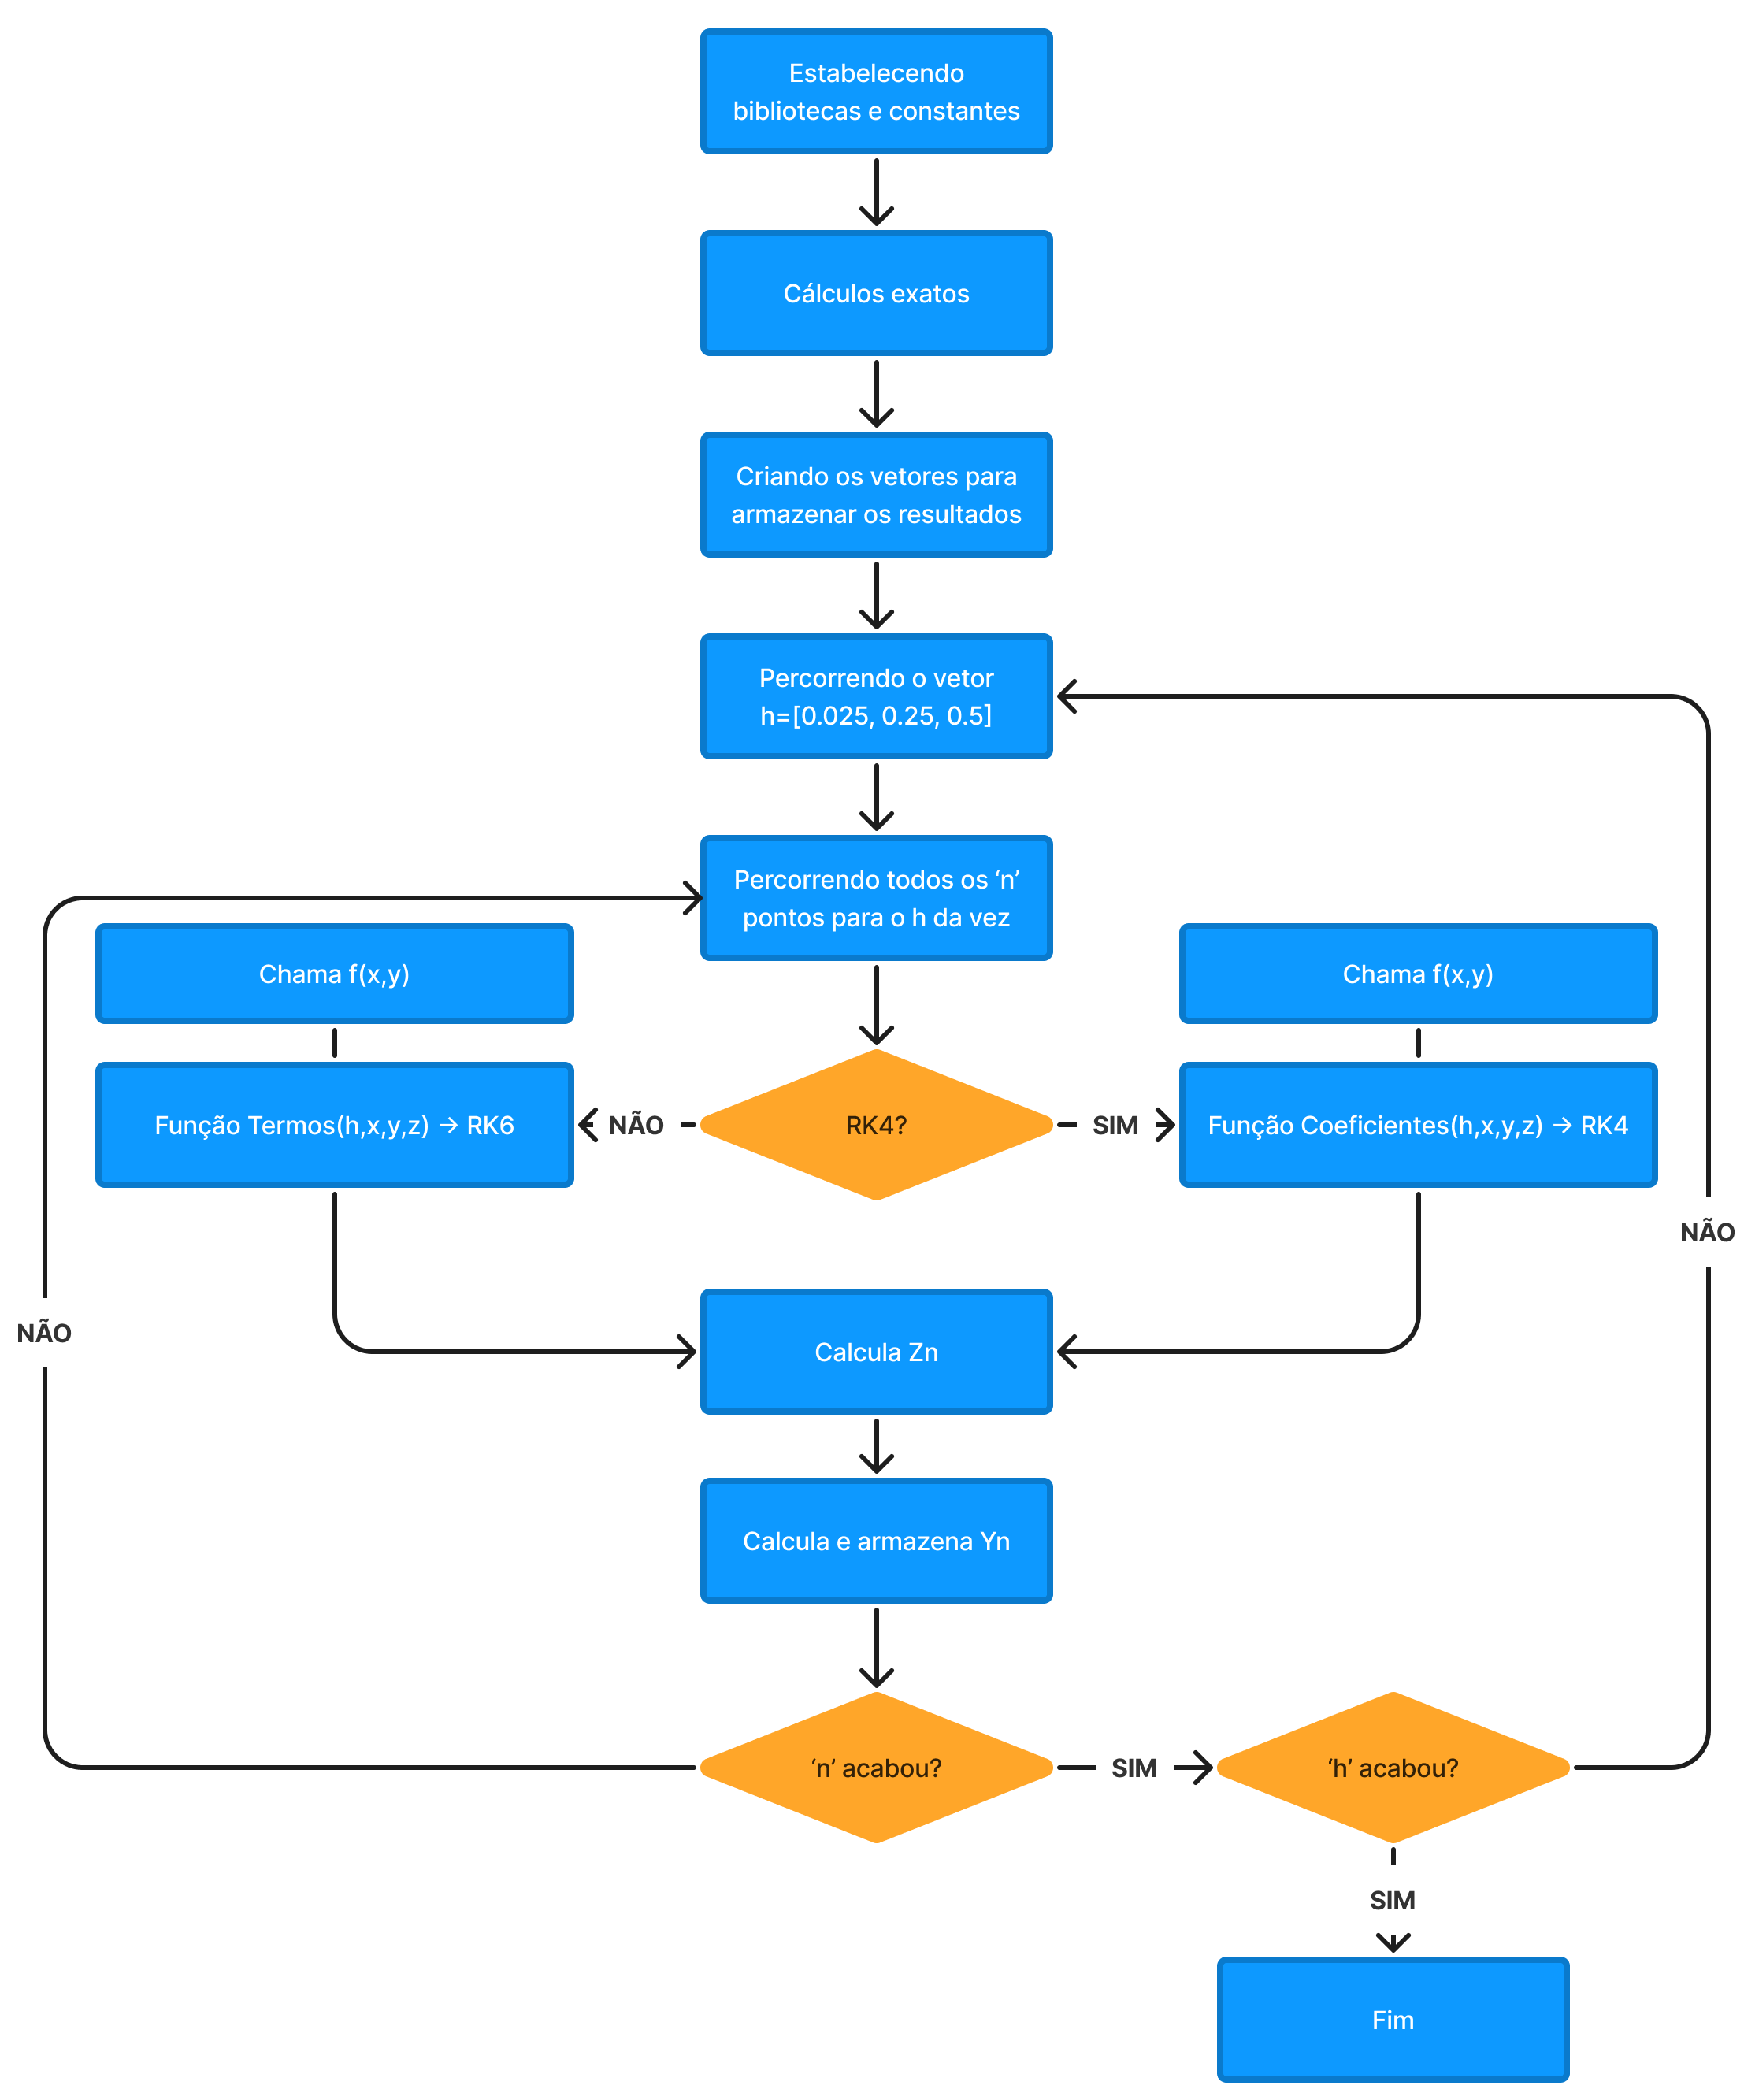
\includegraphics[scale=0.35]{images/Untitled (3).png}}
        \caption[width=\columnwidth]{Fluxo do código em Python.}
        \label{fluxograma}
    \end{figure}

\subsection{Resultados}

    A partir dos gráficos gerados, tanto no Excel quanto no Python, notou-se que tanto para o RK4 quanto para o RK6, a exatidão é prejudicada à medida que o $h$ aumenta. Analisando somente o RK4, nota-se pela figura \ref{RK41} que para o $h$ de 0.025, gráficos da primeira coluna, a curva do resultado exato, curva em cinza, e da solução numérica, curva tracejada em azul, se sobrepõem, denotando uma alta eficiência. Todavia, para os gráficos das segunda e terceira colunas, $h$ de 0.25 e 0.5 respectivamente, as curvas citadas não coincidem em quase nenhum ponto, a não ser para um intervalo muito próximo do início das curvas. Vale ressaltar que para os gráficos da linha de cima da figura, a curva exata foi gerada usando os mesmos valores de $x$ da solução numérica, já na segunda linha as curvas exatas foram geradas usando um $x$ variando pouco de um para outro.
    
    \begin{figure}[H]
        \centering
        \makebox[\textwidth]{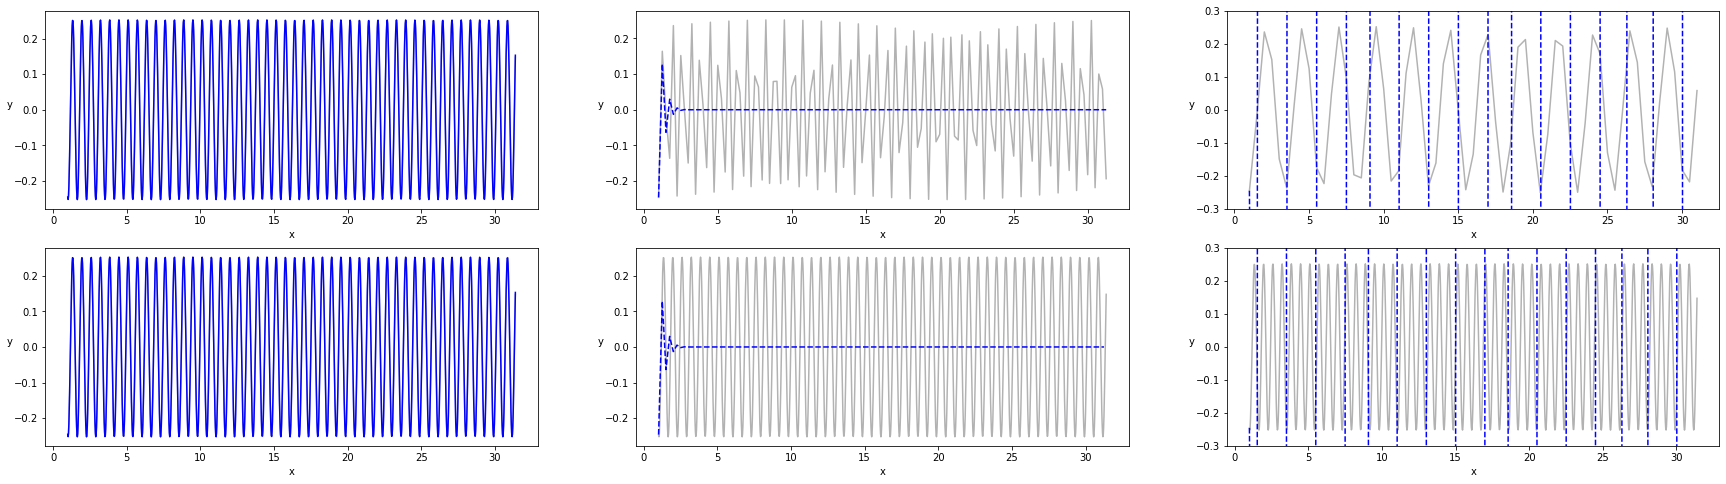
\includegraphics[scale=0.3]{images/RK41.png}}
        \caption[width=\columnwidth]{Variação das soluções do RK4 para h sendo 0.025, 0.25 e 0.5.}
        \label{RK41}
    \end{figure}
    
    Analogamente, para o RK6 (curvas tracejadas em marrom) o fenômeno acontece de forma parecida como observado na figura \ref{RK61}.
    
    \begin{figure}[H]
        \centering
        \makebox[\textwidth]{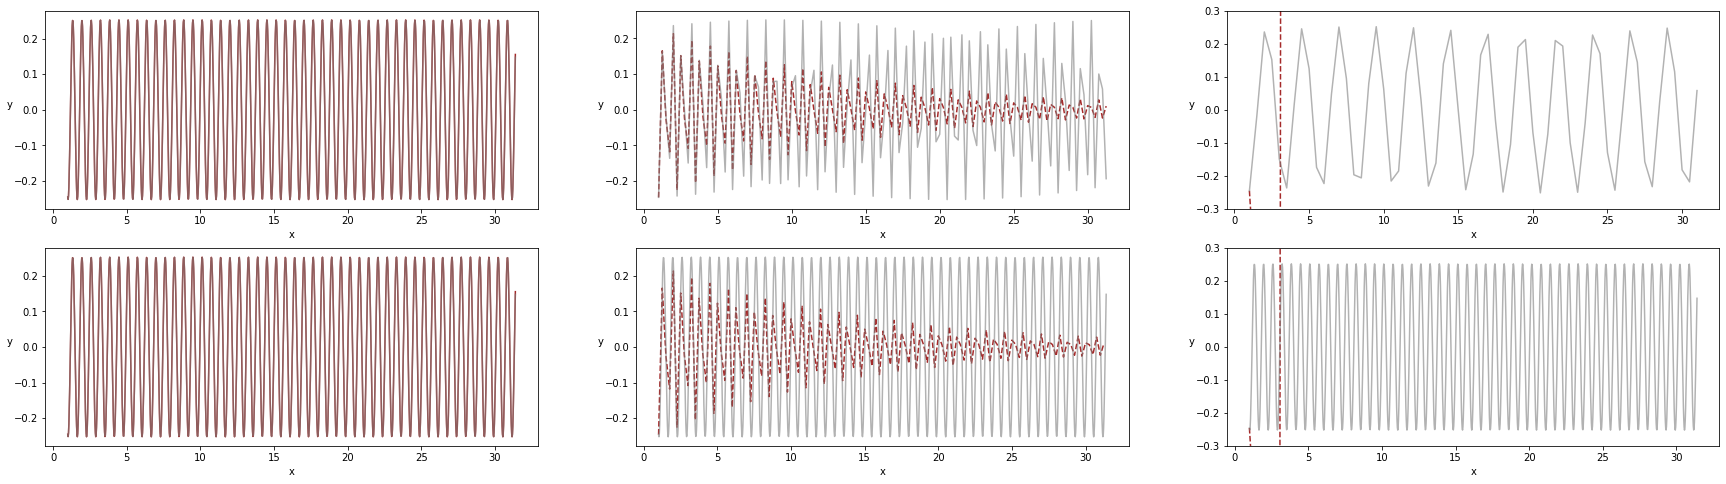
\includegraphics[scale=0.3]{images/RK61.png}}
        \caption[width=\columnwidth]{Variação das soluções do RK6 para h sendo 0.025, 0.25 e 0.5.}
        \label{RK61}
    \end{figure}
    
    Comparando os dois métodos, percebe-se que, muito embora a exatidão diminua com o aumento do $h$, o método do RK6 persiste fiel por mais tempo a solução exata, haja vista que para o $h$ de 0.25 (segunda linha da figura \ref{comp1}), o RK6 (curvas da segunda coluna) poderia ser utilizado para um intervalo maior que o RK4 (curvas da primeira coluna).
    
    \begin{figure}[H]
        \centering
        \makebox[\textwidth]{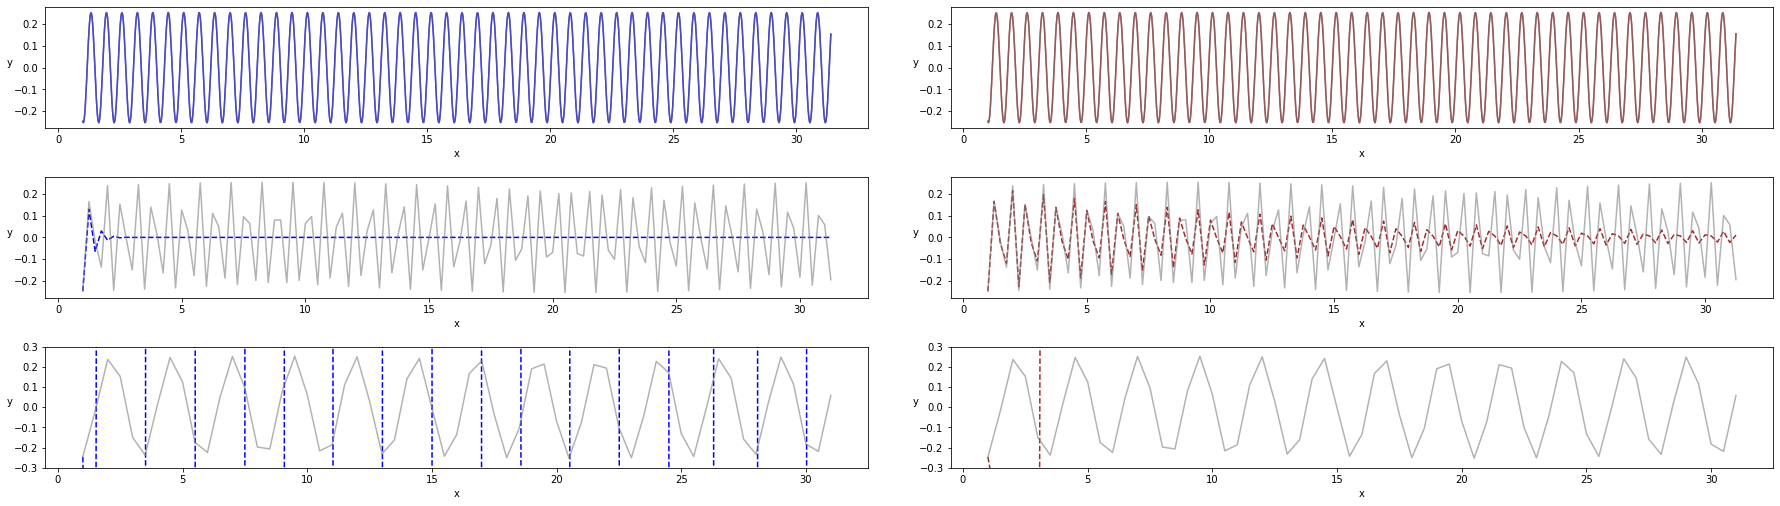
\includegraphics[scale=0.3]{images/comp1.png}}
        \caption[width=\columnwidth]{Comparação RK4 e RK6.}
        \label{comp1}
    \end{figure}
    
    Isso se torna ainda mais perceptível ao se comparar o RK4 e o RK6 com a curva exata com uma variação muito pequena de $x$, observar figura \ref{comp2}.
    
    \begin{figure}[H]
        \centering
        \makebox[\textwidth]{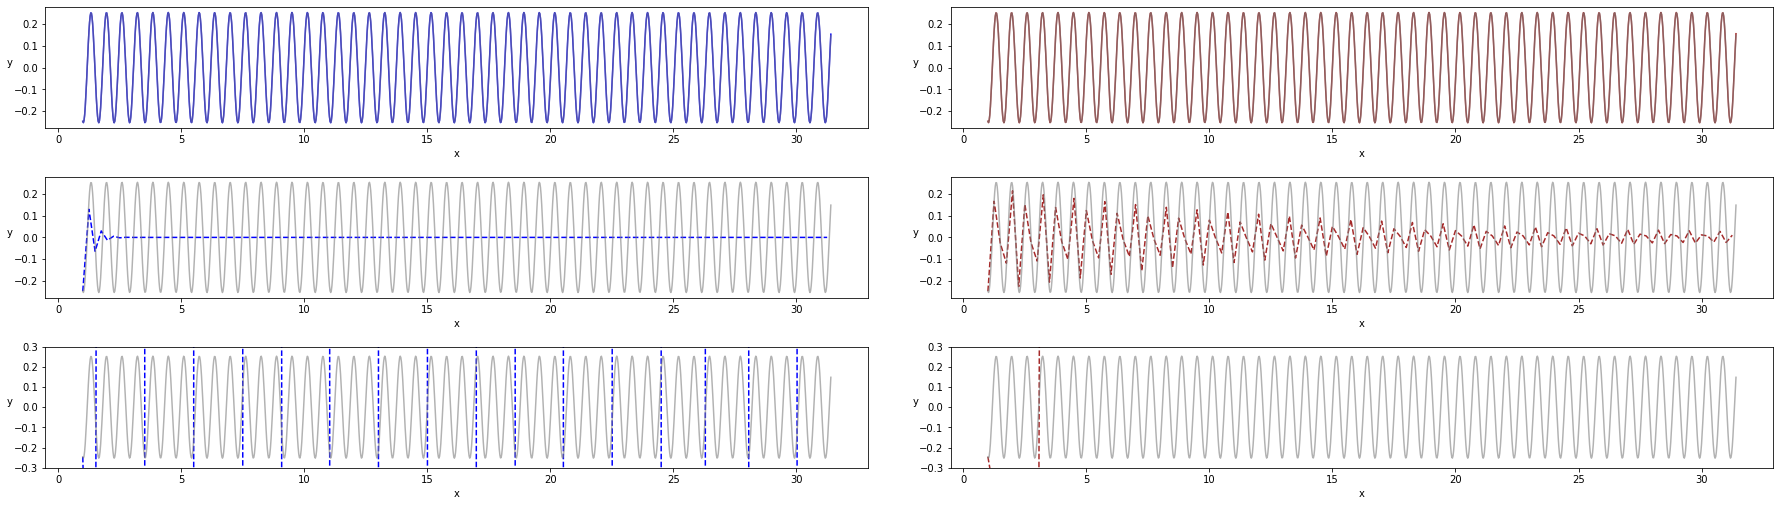
\includegraphics[scale=0.3]{images/comp2.png}}
        \caption[width=\columnwidth]{Comparação RK4 e RK6 com a curva exata.}
        \label{comp2}
    \end{figure}
    
    Para melhor visualizar o impacto da variação do $h$, criou-se uma aplicação Python e disponibilizou-se na plataforma Streamlit para que de forma interativa se possa observar esse impacto para o RK4 e o RK6, observar figura \ref{streamlit}. A aplicação pode ser acessada pelo link \url{https://share.streamlit.io/alanldm/projeto_runge_kutta/metodos.py}.
    
    \begin{figure}[H]
        \centering
        \makebox[\textwidth]{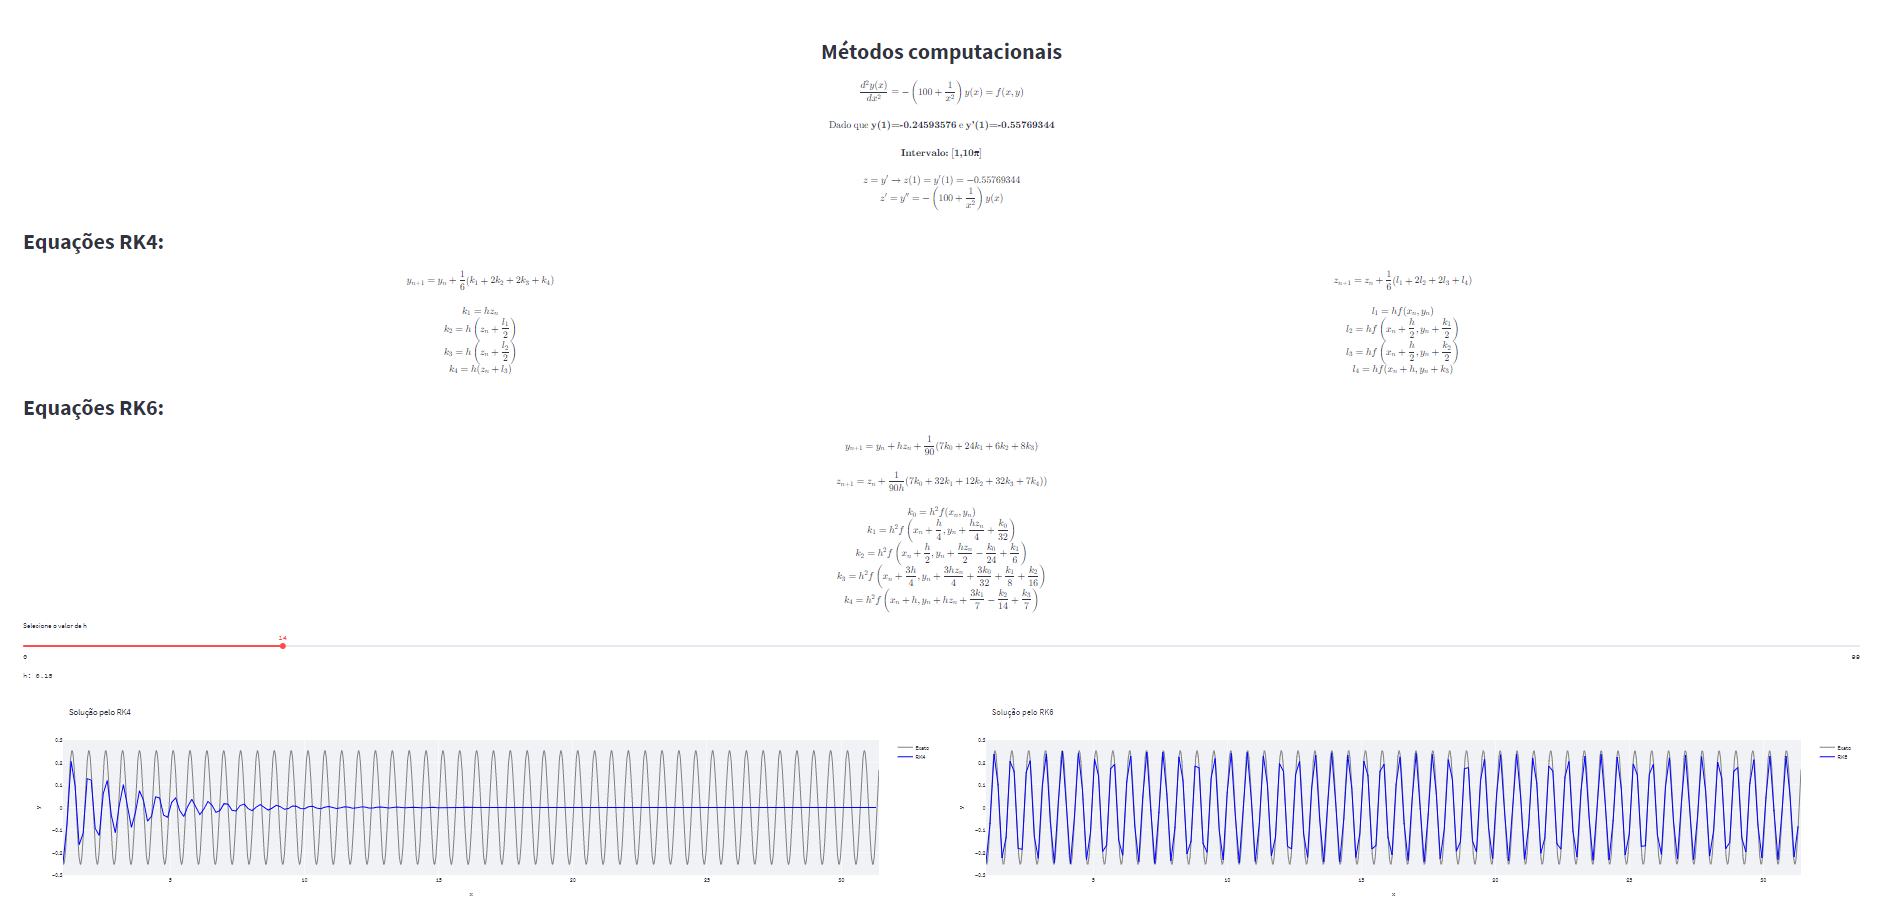
\includegraphics[scale=0.3]{images/streamlit.png}}
        \caption[width=\columnwidth]{Aplicação Python para os métodos RK4 e RK6. Acessar com o link \url{https://share.streamlit.io/alanldm/projeto_runge_kutta/metodos.py}.}
        \label{streamlit}
    \end{figure}
    
    Por fim, um vídeo foi produzido para se verificar essa variação de forma mais rápida. Ele pode ser visto no link citado acima ou no próprio notebook Python disponibilizado.

\subsection{Conversões}

    Utilizando como código guia o programa em Python, as soluções foram convertidas para as linguagens apresentadas na figura \ref{fluxo}. Isto é, as soluções foram passadas também para Julia, C++ e Matlab. O código em Julia foi desenvolvido utilizando a IDE Visual Studio Code (VSCode), em C++ no ambiente de desenvolvimento Repl.it e em Matlab na sua própria IDE. 
    
    
    As maiores dificuldades para essas conversões foram as adaptações de sintaxe e mudanças nas bibliotecas utilizadas. Ademais, a manipulação de vetores em cada linguagem também representou uma barreira. Cabe ressaltar que as repostas em cada linguagem foram comparadas com os resultados em Python e Excel, que foram desenvolvidos independentemente, e todas foram iguais. Sendo assim, garantiu-se a redundância dos resultados e comprovação de seus valores.

\pagebreak

\section{Conclusão}

    Diante do exposto, conclui-se que os métodos de solução numérica RK4 e RK6 são muito precisos para um $h$ muito pequeno, servindo muito bem como uma solução alternativa às integrais. Além disso, com este projeto, pôde-se estudar melhor outras linguagens de programação, bem como verificar a aplicação dos conhecimentos da disciplina de métodos computacionais em diferentes linguagens. Exercitou-se ainda a construção de aplicações Python, bem como o desenvolvimento de gráficos nessa linguagem e em Excel.

\pagebreak


\nocite{Overleaf}
\nocite{Julia_Operadores}
\nocite{Julia_Introducao}
\nocite{Julia_Data_Frame}
\nocite{Julia_arrays}
\nocite{Julia_funcoes}
\nocite{Matplotlib}
\nocite{Deploy}
\nocite{Stcolumns}
\nocite{Stvideo}
\nocite{Ar}
\nocite{API}
\nocite{Stlatex}
\nocite{Cplusplus}


\printbibliography



\end{document}
